% !TEX root = ../main.tex

\section{Introduction}
Ethereum project\cite{Ref00} launched in 2014 by introducing Ether as its protocol-level cryptocurrency. It is ranked second in terms of market value after Bitcoin.\footnote{CoinMarketCap - Ethereum currency - Accessed: 2019-02-11 \newline\url{https://coinmarketcap.com/currencies/ethereum/}} Ethereum has the biggest development community to track enhancement and propose new ideas.\footnote{CoinDesk Crypto-Economics Explorer - Accessed: 2019-02-11 \newline\url{https://www.coindesk.com/data}} It offers an ecosystem to implement any type of distributed application on the blockchain. Tokens are essential part of this ecosystem which define set of rules---known as API\footnote{Advanced Programming Interface.}---for standardizing interaction with smart contracts.\footnote{Types of transactions that execute as they are programmed by Ethereum scripting language (e.g., Solidity or Vyper)}. Therefore, any ERC20\footnote{ERC20 is title of the standard and it should be referred as EIP20 (which is the actual proposal for improvement). In this paper we use both ERC20 and EIP20 in one sense for simplicity.}-compliant application can interact with any ERC20 token. For example, shares of company X can be represented as ERC20 tokens to be reusable by other smart contracts (e.g., online exchanges, automated payment systems, decentralized games, etc). Leveraging ERC20 token facilitates implementation of financial assets while raising some security concerns. ERC20 tokens are technically standardized version of smart contracts that could be similarly vulnerable to security flaws.
\begin{figure}[t]
	\centering
	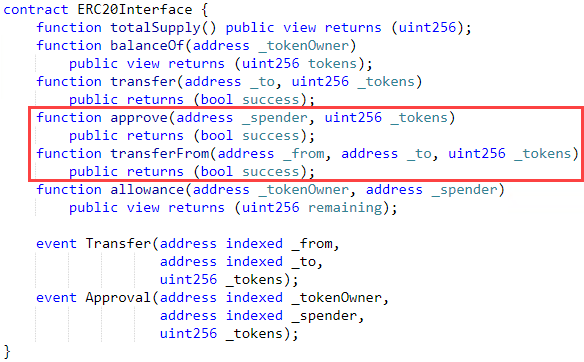
\includegraphics[width=1.0\linewidth]{figures/multiple_withdrawal_01.png}
	\caption{Importance of ERC20 security in case of (1) digitizing share of company X (2) representing a fiat currency. In this case, smart contracts interact with two different ERC20 tokens which are repressing in order, a financial instrument and a non-collateralized stablecoin. Any security vulnerability in written code of ERC20 tokens, will impact security of related smart contracts and value of underlying assets.}
\end{figure}

Since introduction of ERC20 standard in November 2015, several vulnerabilities have been discovered and addressed by Ethereum community. In October 2017, a new security issue---known as "Multiple Withdrawal Attack"---opened on GitHub\cite{Ref13,Ref07}. The attack originating from definition of two interfaces\footnote{Interface defines parameters and expected outputs of each function without implementing them. Developers are free to write arbitrary codes that could potentially lead to a security issue.} in ERC20 standard for approving and transferring tokens. Using these functions in an undesirable situation (e.g., front-running) could result in conditions that tokens being spent by another third party on behalf of the owner. This issue is still open and several solutions have been made to mitigate it. In this paper we examine 10 suggested solutions in terms of compatibility with the standard and attack mitigation. Since none of them could satisfy constraints of ERC20 standard, we motivated to introduce a new solution to mitigate the attack.

Authors of ERC20 standard \cite{Ref08}, provided generic implementations of ERC20 tokens from OpenZeppelin\cite{Ref10} and ConsenSys\cite{Ref11}. OpenZeppelin uses two additional methods and ConsenSys has not attempted to work around the issue. There are other implementations that have different trade-offs. We compared them in the below table and they violate constraints of the standard. The attack could happen because of a gap between transactions. Our solution addresses this gap by using compare and set (CAS) pattern\cite{Ref06}. CAS is one of the most widely used lock-free synchronization strategy that allows comparing and setting values in an atomic way. It allows to compare values in one transaction and set new values before transferring control to another one. We leveraged this pattern to remove gap between transactions and prevent race condition as root cause of the attack.

\begin{figure}[H]
	\centering
	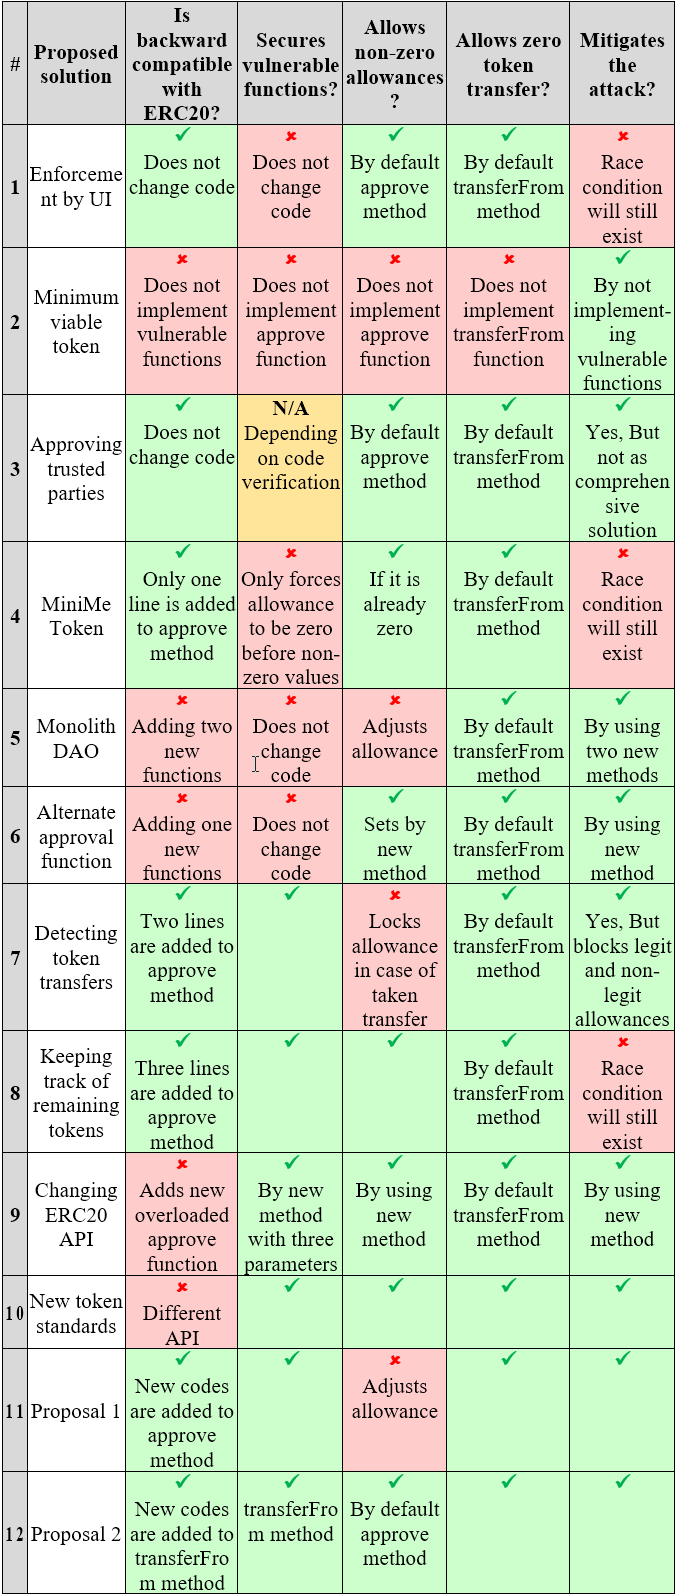
\includegraphics[width=1.0\linewidth]{figures/multiple_withdrawal_04.png}
	\caption{Comparison of 10 suggested solutions with two proposals contributed by this paper. Proposal 2 uses CAS pattern to mitigate the attack sustainably by (1) comparing transferred tokens through a new local variable in \textit{transferFrom} function and (2) tracking of transferred tokens for preventing more transfers in the next transaction.}
\end{figure}